\section{Aplikace}
Aplikace je napsaná v~nativním C++--11, ve vývojovém prostředí Visual Studio 2015. Jedná se o~multiplatformní konzolovou aplikaci, která byla primárně určena pro systémy ARM s~operačním systémem Linux. Hlavním účelem této aplikace je detekování chodců v~obrazech.

Její obsluha je na bázi argumentů, které určují její chování. Nastavení parametrů se provádí přes externí soubor, což umožňuje jednodušší a~pohodlnější manipulaci s~aplikací. Disponuje širokým spektrem nástrojů od testování klasifikátorů, po jejich trénování až po samotnou detekci. Její nástroje jsou popsány v~následujících podsekcích.

\subsection{Detekování chodců}
Aplikace umožnuje detekování chodců ve videosekvencích, obrázcích a~také z~webové kamery. Díky externímu nastavení prahů detektorů a~jiných proměnných lze měnit nastavení bez opětovného kompilování aplikace. Součástí aplikace je anotační nástroj, který slouží k~označení oblasti s~chodci. Nástroj zaznamená výstup do souboru, kterým se vyhodnotí výstup detektoru.
 
Obrázek \ref{mog_algorithm} ilustruje průběh algoritmu při volbě detekce pomocí metody MOG a~HOG. Prvním krokem algoritmu je získání snímku z~aktuální videosekvence nebo kamery (getFrame), pokud obrázek je prázdný, cyklus zde končí. Snímek se následně předzpracovává převodem do stupňů šedi a~aplikací filtru rozostření (preprocessing). Tento obrázek je následně zpracováván metodikou substrakce pozadí (mogMask) a~na tento obraz se aplikuje eroze a~dilatace(erodeDilate), proto, aby se v~snímku vyfiltrovaly malé, nevýznamné oblasti a~následně spojily ty větší potencionální, kde se může nacházet chodec. Tyto oblasti se obalí pomocí kontur a~převedou se na obdélníky (wrapObject), díky kterým se z~obrazu vystřihnou tyto části (cropFrame). Na získaných oblastech v~následujícím kroku probíhá samotná detekce (detect). Detekční metoda vrátí obdélníkové oblasti potencionálních chodců a~vykreslí je do původního obrazu (drawRects). Proces se opakuje do té doby, dokud získaný obrázek z~kamery není prázdný. Pokud obrázek po aplikování masky substrakce pozadí neobsahuje dostatečně velké oblasti k~aplikaci rámců, program pokračuje načítáním dalšího obrazce z~kamery.  

\begin{figure}[H]
\centering
\includegraphics[width=14cm]{figures/alg_moghog}
\caption{Algoritmus aplikace při selekci kombinace MOG a~HOG detekce}
\label{mog_algorithm}
\end{figure}

\subsection{Křížová validace klasifikátoru}
Křízová validace (cross validation) je metoda zjišťování, jak moc bude daný klasifikátor spolehlivý v~pozitivní detekci. Vytrénovaný klasifikátor se otestuje na sadě vzorků, které nebyly součástí jeho tréninku a~známe jejich přesnou kategorii zařazení.

Aplikace nabízí křížovou validaci OpenCV a~Dlib klasifikátoru. Diskriminační klasifikátor SVM z~OpenCV lze validovat třemi způsoby. První je náhodný přístup, generování trénovacích parametrů klasifikátoru s~různou iterací.

Další efektivnějším způsobem validace je pomocí diferenciální evoluce. Tento algoritmus vychází z~genetického žíhání. Algoritmus nastaví určitý počet dimenzí pro validaci parametrů SVM a~následně probíhá \uv{žíhání} parametrů takřka k~jejich dokonalosti. Tento proces trvá 1000 cyklů.

Posledním druhem validace pro klasifikátor SVM z~OpenCV je podobný z~Dlib knihovny, jedná se o~vnořené cykly, kde se hrubou silou postupně testují parametry a~výsledek validace se vypisuje do konzole. 

Pro klasifikátor z~Dlib knihovny je použita pouze metodika pro postupné testování parametrů hrubou silou v~cyklech, která je dostupná v~knihovně. Výhodou této validace je rozdělení trénovacích dat do 3 množin, kde dvě slouží na trénování a~jedna pro testování a~následně se prohodí. Čímž zajistíme větší přesnost trénovacích parametrů. Tato validace má nejdelší výpočetní čas a~jejím výsledkem je přesnost klasifikátoru pro pozitivní a~negativní množinu vzorků.

\subsection{Testování klasifikátoru}
Testování klasifikátoru je proces, při kterém se otestuje na daných trénovacích vzorcích, u~kterých známe jejich třídu. Díky této metodice zjistíme, jak spolehlivě je vytrénovaná SVM a~jaká je její přesnost detekce. Přesněji řečeno k~daným vzorkům máme soubor \uv{ground truth} hodnot, proti kterým se porovnává výstup predikce daného klasifikátoru. 

\subsection{Trénování klasifikátoru}
Program také umožňuje vytrénování vlastního klasifikátoru. Parametry se vyberou z~externího souboru s~nastavením. V~tomto souboru jsou také uloženy cesty k~souborům se vzorky. 

Trénovací režim aplikace lze spustit přes argument '-t=train" a~následně je uživateli nabídnut typ trénování. Program zvládne vytrénovat klasifikátor jak z~knihovny OpenCV, tak i~z~knihovny Dlib. 

Trénování klasifikátorů z~OpenCV probíhá naplněním vzorků do paměti včetně jejich kategorizace. Následně pro každý vzorek jsou vypočítané jeho příznaky a~opět jsou uloženy do paměti programu. Posledním krokem před trénováním je jejich převod do jednořádkové matice a~poté je spuštěno samotné trénování klasifikátorů. Tento krok trvá v~závislosti na velikosti trénovací matice a~zvolených parametrů. Uživatel může zvolit i~dvojité trénování, což je stejný postup, ale na konci trénování se spustí detekce pomocí posuvného okna na negativních vzorcích a~tyto vzorky budou rozšířeny o~výstup z~detektoru. Tento proces se nazývá Bootstraping. Výstupem trénování je soubor YAML, který je strojově čitelný a~slouží pro serializaci strukturovaných dat. Nalezneme zde parametry, použité pro trénování, vytrénované vzorky a~vektor, který určuje rozdělující přímku.

Další možností je vytrénování klasifikátoru z~knihovny Dlib. Trénování je obdobné jako u~předchozí metody. %Data jsou načtena jako mapy obrázků a~tyto obrázky se parsují pomocí XML souboru. Trénování probíhá pouze z~pozitivních vzorků. 

Poslední možností trénování je kombinace výše zmíněných postupů. Vzorky se zpracují za pomocí OpenCV knihovny a~vstupem do trénovací metody klasifikátoru z~knihovny Dlib je trénovací matice. Tu je nejprve nutné převést na formát této knihovny a~poté je možné provést samotné trénování.
Výstupem trénovací metody z~knihovny Dlib je binární soubor.
%Podstatný rozdíl mezi těmito binárními klasifikátory je v~rozdílu jejich štítku. OpenCV klasifikátor můžeme definovat štítky libovolně, nejčastější však $1$ pro pozitivní vzorky a~$0$ pro negativní. Zatím co Dlib klasifikátor přijímá pouze $1$ pro pozitivní a~$-1$ pro negativní vzorky.

Trénování klasifikátoru je velmi náročnou operací na hardwarové prostředky. Ovšem závisí na trénovací sadě. Sada o~počtu 200 tisíc vzorků zkonzumuje až 16 GB paměti.

\subsection{Anotace chodců v~obraze} Do výsledného programu jsem naimplementoval nástroj pro anotaci chodců v~obraze. Pomocí tohoto nástroje můžeme anotovat až 5 chodců (každá anotace má svou barvu).
Při vývoji jsem se snažil o~to, aby manipulace s~tímto nástrojem byla jednoduchá a~intuitivní. Náhled nástroje je na obrázku \ref{tool_anotate}.
%Aplikace také disponuje nástrojem pro anotaci chodců v~obraze. Najednou umožňuje anotovat až 5 chodců a~tyto anotace, i~když to není až tak potřebné pro správnost anotace, jsou od sebe barevně odlišeny. Manipulace s~tímto nástrojem je velmi snadná a~jeho náhled je na obrázku \ref{tool_anotate}.
Anotovaná část se může překrývat s~jinou. Konkrétní anotace je zobrazena pro kontrolu samostatně zobrazena v~dalším okně.
Všechny tyto objekty zájmu a~snímek s~anotacemi jsou uloženy na disk v~podobě obrázku pro pozdější kontrolu nebo objekty zájmu mohou být použity jako pozitivní vzorky pro trénování nebo křížovou validaci klasifikátoru. Výstup tohoto nástroje je plně kompatibilní s~evaluační funkcí programu a~jedná se tedy o~\uv{ground truth} soubor všech anotací objektů zájmu ve videosnímku. Stručný manuál k~nástroji je popsán v~příloze \ref{manual}.
 \begin{figure}[H]
\centering
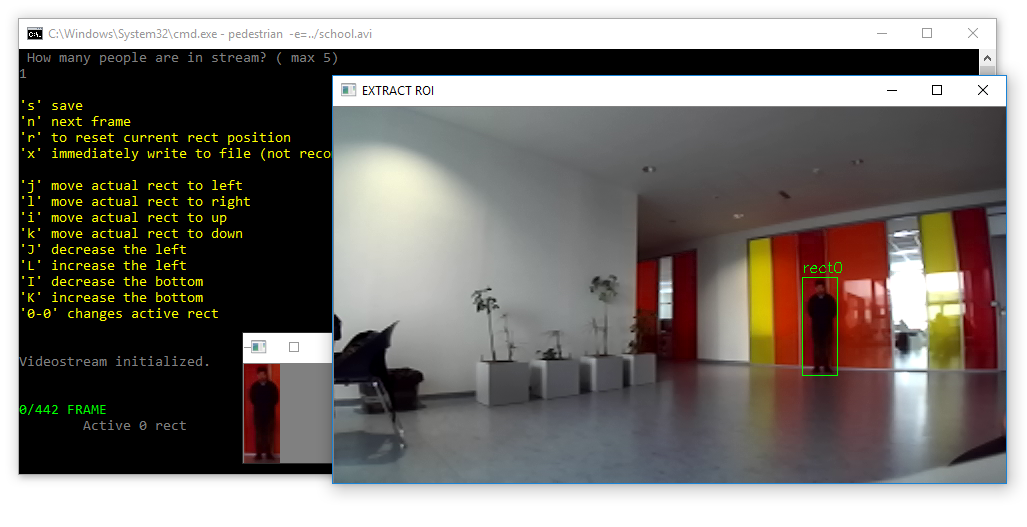
\includegraphics[width=16cm]{figures/annotation_example}
\caption{Nástroj pro anotování oblastí chodců}
\label{tool_anotate}
\end{figure}

\subsection{Tvorba negativních vzorků z~obrazu}
Tento nástroj umožňuje vytvořit negativní vzorky pro trénování procházením obrázku pomocí posuvného okna. Velikost posuvného okna je definována v~externím souboru. Vstupem je textový soubor s~cestami k~obrázkům.

%Nástroj popsaný v předchozí kapitole také umožnuje vytvořit negativní vzorky.


%% připdat výpis z GT